% Learned-query resampler funnel — TikZ source. Compiles to a tight standalone
% PDF (pdflatex figures/resampler-funnel.tex), which `book-scaffold build-figures`
% converts to public/figures/resampler-funnel.svg (PDF -> SVG via pdftocairo).
%
% n visual features (left) are cross-attended by m learned latent queries
% (middle, parameters) into a FIXED m soft tokens (right), regardless of n.
\documentclass[tikz,border=3pt]{standalone}
\usepackage{amsmath}
\usepackage{amssymb}
\usepackage{tikz}
\usetikzlibrary{positioning,arrows.meta,calc,fit}
\begin{document}
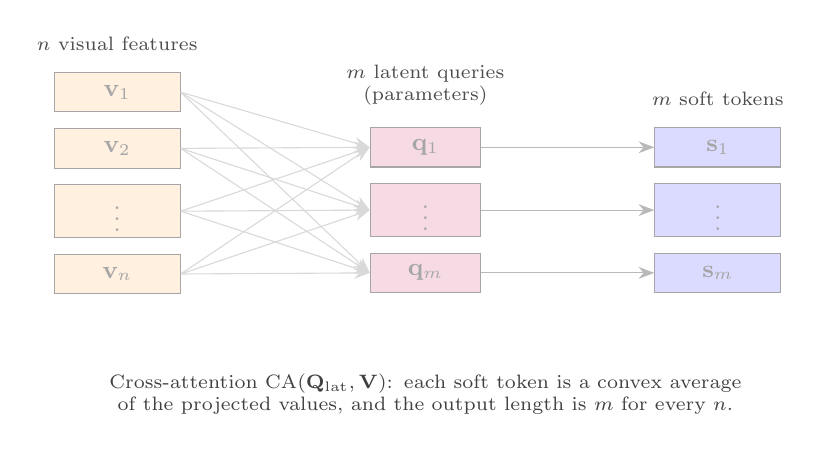
\begin{tikzpicture}[
    font=\small,
    feat/.style={draw, gray!70, fill=orange!12, minimum width=16mm,
                 minimum height=5mm, inner sep=2pt},
    qry/.style={draw, gray!70, fill=purple!14, minimum width=14mm,
                minimum height=5mm, inner sep=2pt},
    tok/.style={draw, gray!70, fill=blue!14, minimum width=16mm,
                minimum height=5mm, inner sep=2pt},
    op/.style={->, >={Stealth[length=2.0mm]}, gray!55},
  ]
  % --- n visual features (left, tall) ---
  \node[feat] (v1) {$\mathbf v_1$};
  \node[feat, below=2mm of v1] (v2) {$\mathbf v_2$};
  \node[feat, below=2mm of v2] (vd) {$\vdots$};
  \node[feat, below=2mm of vd] (vn) {$\mathbf v_n$};
  \node[above=1.5mm of v1, font=\scriptsize, text=black!70]
    {$n$ visual features};

  % --- m latent queries (middle) ---
  \node[qry, right=24mm of v1, yshift=-7mm] (q1) {$\mathbf q_1$};
  \node[qry, below=2mm of q1] (q2) {$\vdots$};
  \node[qry, below=2mm of q2] (qm) {$\mathbf q_m$};
  \node[above=1.5mm of q1, font=\scriptsize, text=black!70, align=center]
    {$m$ latent queries\\(parameters)};

  % cross-attention edges (funnel)
  \foreach \v in {v1,v2,vd,vn}
    \foreach \q in {q1,q2,qm}
      \draw[op, gray!30] (\v.east) -- (\q.west);

  % --- m soft tokens (right) ---
  \node[tok, right=22mm of q1] (s1) {$\mathbf s_1$};
  \node[tok, below=2mm of s1] (s2) {$\vdots$};
  \node[tok, below=2mm of s2] (sm) {$\mathbf s_m$};
  \node[above=1.5mm of s1, font=\scriptsize, text=black!70]
    {$m$ soft tokens};

  \draw[op] (q1.east) -- (s1.west);
  \draw[op] (q2.east) -- (s2.west);
  \draw[op] (qm.east) -- (sm.west);

  \node[below, align=center, text width=9cm, font=\scriptsize, text=black!75]
    at ($(qm.south)+(0,-0.9)$)
    {Cross-attention $\operatorname{CA}(\mathbf Q_{\mathrm{lat}},\mathbf V)$: each soft
     token is a convex average of the projected values, and the output length is
     $m$ for every $n$.};
\end{tikzpicture}
\end{document}
